\documentclass[tikz,border=6pt]{standalone}
\usepackage{amsmath,amssymb}
\usepackage{xcolor}
\definecolor{accent}{HTML}{A13D2C}
\definecolor{accent2}{HTML}{2B5F6B}
\definecolor{muted}{HTML}{5A564F}
\definecolor{linecol}{HTML}{D8D2C4}
\definecolor{astroblue}{HTML}{1B4F72}
\definecolor{sunyellow}{HTML}{E8A33D}
\usetikzlibrary{calc,arrows.meta}
\begin{document}
% A star passes a field star (centre) at impact parameter b along a straight line.
% The cylinder of radius b about the axis through the field star, parallel to the path, contains the path.
% Pull arrows point from points of the path to the field star, length proportional to 1/distance^2.
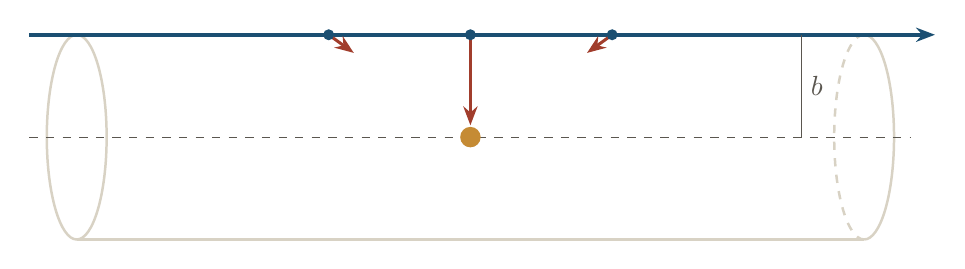
\begin{tikzpicture}[x=1cm,y=1cm, >={Stealth[length=2.4mm]}]
  \def\b{1.3}
  % cylinder
  \draw[linecol, line width=0.9pt] (-5,\b) -- (5,\b);
  \draw[linecol, line width=0.9pt] (-5,-\b) -- (5,-\b);
  \draw[linecol, line width=0.9pt] (-5,0) ellipse (0.38 and \b);
  \draw[linecol, line width=0.9pt] (5,-\b) arc (-90:90:0.38 and \b);
  \draw[linecol, line width=0.9pt, dashed] (5,\b) arc (90:270:0.38 and \b);
  \draw[muted, dashed] (-5.6,0) -- (5.6,0);
  % the path, on the top of the cylinder
  \draw[->, astroblue, line width=1.3pt] (-5.6,\b) -- (5.9,\b);
  % impact parameter
  \draw[muted] (4.2,0) -- (4.2,\b) node[midway, right] {$b$};
  % pulls from three points of the path: (x,b) -> towards (0,0), length 1.0*(b^2/(b^2+x^2))
  \foreach \x in {-1.8,0,1.8} {
    \pgfmathsetmacro{\d}{sqrt(\x*\x+\b*\b)}
    \pgfmathsetmacro{\L}{1.15*\b*\b/(\d*\d)}
    \draw[->, accent, line width=1.1pt] (\x,\b) -- ($(\x,\b)!\L cm!(0,0)$);
    \fill[astroblue] (\x,\b) circle (0.07);
  }
  \fill[sunyellow!85!black] (0,0) circle (0.13);
\end{tikzpicture}
\end{document}
